\documentclass[twoside]{book}

% Packages required by doxygen
\usepackage{fixltx2e}
\usepackage{calc}
\usepackage{doxygen}
\usepackage[export]{adjustbox} % also loads graphicx
\usepackage{graphicx}
\usepackage[utf8]{inputenc}
\usepackage{makeidx}
\usepackage{multicol}
\usepackage{multirow}
\PassOptionsToPackage{warn}{textcomp}
\usepackage{textcomp}
\usepackage[nointegrals]{wasysym}
\usepackage[table]{xcolor}

% Font selection
\usepackage[T1]{fontenc}
\usepackage[scaled=.90]{helvet}
\usepackage{courier}
\usepackage{amssymb}
\usepackage{sectsty}
\renewcommand{\familydefault}{\sfdefault}
\allsectionsfont{%
  \fontseries{bc}\selectfont%
  \color{darkgray}%
}
\renewcommand{\DoxyLabelFont}{%
  \fontseries{bc}\selectfont%
  \color{darkgray}%
}
\newcommand{\+}{\discretionary{\mbox{\scriptsize$\hookleftarrow$}}{}{}}

% Page & text layout
\usepackage{geometry}
\geometry{%
  a4paper,%
  top=2.5cm,%
  bottom=2.5cm,%
  left=2.5cm,%
  right=2.5cm%
}
\tolerance=750
\hfuzz=15pt
\hbadness=750
\setlength{\emergencystretch}{15pt}
\setlength{\parindent}{0cm}
\setlength{\parskip}{3ex plus 2ex minus 2ex}
\makeatletter
\renewcommand{\paragraph}{%
  \@startsection{paragraph}{4}{0ex}{-1.0ex}{1.0ex}{%
    \normalfont\normalsize\bfseries\SS@parafont%
  }%
}
\renewcommand{\subparagraph}{%
  \@startsection{subparagraph}{5}{0ex}{-1.0ex}{1.0ex}{%
    \normalfont\normalsize\bfseries\SS@subparafont%
  }%
}
\makeatother

% Headers & footers
\usepackage{fancyhdr}
\pagestyle{fancyplain}
\fancyhead[LE]{\fancyplain{}{\bfseries\thepage}}
\fancyhead[CE]{\fancyplain{}{}}
\fancyhead[RE]{\fancyplain{}{\bfseries\leftmark}}
\fancyhead[LO]{\fancyplain{}{\bfseries\rightmark}}
\fancyhead[CO]{\fancyplain{}{}}
\fancyhead[RO]{\fancyplain{}{\bfseries\thepage}}
\fancyfoot[LE]{\fancyplain{}{}}
\fancyfoot[CE]{\fancyplain{}{}}
\fancyfoot[RE]{\fancyplain{}{\bfseries\scriptsize Generated by Doxygen }}
\fancyfoot[LO]{\fancyplain{}{\bfseries\scriptsize Generated by Doxygen }}
\fancyfoot[CO]{\fancyplain{}{}}
\fancyfoot[RO]{\fancyplain{}{}}
\renewcommand{\footrulewidth}{0.4pt}
\renewcommand{\chaptermark}[1]{%
  \markboth{#1}{}%
}
\renewcommand{\sectionmark}[1]{%
  \markright{\thesection\ #1}%
}

% Indices & bibliography
\usepackage{natbib}
\usepackage[titles]{tocloft}
\setcounter{tocdepth}{3}
\setcounter{secnumdepth}{5}
\makeindex

% Custom commands
\newcommand{\clearemptydoublepage}{%
  \newpage{\pagestyle{empty}\cleardoublepage}%
}

\usepackage{caption}
\captionsetup{labelsep=space,justification=centering,font={bf},singlelinecheck=off,skip=4pt,position=top}

%===== C O N T E N T S =====

\begin{document}

% Titlepage & ToC
\pagenumbering{alph}
\begin{titlepage}
\vspace*{7cm}
\begin{center}%
{\Large Fuzzy C-\/means in native C++ \\[1ex]\large v1.\+0 }\\
\vspace*{1cm}
{\large Generated by Doxygen 1.8.14}\\
\end{center}
\end{titlepage}
\clearemptydoublepage
\pagenumbering{roman}
\tableofcontents
\clearemptydoublepage
\pagenumbering{arabic}

%--- Begin generated contents ---
\chapter{R\+E\+A\+D\+ME}
\label{md__r_e_a_d_m_e}
Fuzzy c-\/means clustering algorithm 
\chapter{Namespace Index}
\section{Namespace List}
Here is a list of all namespaces with brief descriptions\+:\begin{DoxyCompactList}
\item\contentsline{section}{\textbf{ gf} }{\pageref{namespacegf}}{}
\item\contentsline{section}{\textbf{ mfnc} }{\pageref{namespacemfnc}}{}
\end{DoxyCompactList}

\chapter{Class Index}
\section{Class List}
Here are the classes, structs, unions and interfaces with brief descriptions\+:\begin{DoxyCompactList}
\item\contentsline{section}{\mbox{\hyperlink{class_cluster}{Cluster}} }{\pageref{class_cluster}}{}
\item\contentsline{section}{\mbox{\hyperlink{class_fuzzy_c_means}{Fuzzy\+C\+Means}} }{\pageref{class_fuzzy_c_means}}{}
\item\contentsline{section}{\mbox{\hyperlink{class_point}{Point}} }{\pageref{class_point}}{}
\item\contentsline{section}{\mbox{\hyperlink{class_properties_parser}{Properties\+Parser}} }{\pageref{class_properties_parser}}{}
\end{DoxyCompactList}

\chapter{File Index}
\section{File List}
Here is a list of all files with brief descriptions\+:\begin{DoxyCompactList}
\item\contentsline{section}{\textbf{ Cluster.\+cpp} }{\pageref{_cluster_8cpp}}{}
\item\contentsline{section}{\textbf{ Cluster.\+h} }{\pageref{_cluster_8h}}{}
\item\contentsline{section}{\textbf{ Data\+Types.\+h} }{\pageref{_data_types_8h}}{}
\item\contentsline{section}{\textbf{ Fuzzy\+C\+Means.\+cpp} }{\pageref{_fuzzy_c_means_8cpp}}{}
\item\contentsline{section}{\textbf{ Fuzzy\+C\+Means.\+h} }{\pageref{_fuzzy_c_means_8h}}{}
\item\contentsline{section}{\textbf{ Generic\+Func.\+cpp} }{\pageref{_generic_func_8cpp}}{}
\item\contentsline{section}{\textbf{ Generic\+Func.\+h} }{\pageref{_generic_func_8h}}{}
\item\contentsline{section}{\textbf{ main.\+cpp} }{\pageref{main_8cpp}}{}
\item\contentsline{section}{\textbf{ Math\+Func.\+h} }{\pageref{_math_func_8h}}{}
\item\contentsline{section}{\textbf{ Point.\+cpp} }{\pageref{_point_8cpp}}{}
\item\contentsline{section}{\textbf{ Point.\+h} }{\pageref{_point_8h}}{}
\item\contentsline{section}{\textbf{ Properties\+Parser.\+cpp} }{\pageref{_properties_parser_8cpp}}{}
\item\contentsline{section}{\textbf{ Properties\+Parser.\+h} }{\pageref{_properties_parser_8h}}{}
\item\contentsline{section}{D\+:\textbackslash{}\+Visual\+Studio2015\+Projects\textbackslash{}\+Fuzzy\+C\+Means\textbackslash{}\+Fuzzy\+C\+Means\textbackslash{}doc/html/\textbf{ dynsections.\+js} }{\pageref{dynsections_8js}}{}
\item\contentsline{section}{D\+:\textbackslash{}\+Visual\+Studio2015\+Projects\textbackslash{}\+Fuzzy\+C\+Means\textbackslash{}\+Fuzzy\+C\+Means\textbackslash{}doc/html/\textbf{ jquery.\+js} }{\pageref{jquery_8js}}{}
\item\contentsline{section}{D\+:\textbackslash{}\+Visual\+Studio2015\+Projects\textbackslash{}\+Fuzzy\+C\+Means\textbackslash{}\+Fuzzy\+C\+Means\textbackslash{}doc/html/\textbf{ menu.\+js} }{\pageref{menu_8js}}{}
\item\contentsline{section}{D\+:\textbackslash{}\+Visual\+Studio2015\+Projects\textbackslash{}\+Fuzzy\+C\+Means\textbackslash{}\+Fuzzy\+C\+Means\textbackslash{}doc/html/\textbf{ menudata.\+js} }{\pageref{menudata_8js}}{}
\item\contentsline{section}{D\+:\textbackslash{}\+Visual\+Studio2015\+Projects\textbackslash{}\+Fuzzy\+C\+Means\textbackslash{}\+Fuzzy\+C\+Means\textbackslash{}doc/html/\textbf{ navtree.\+js} }{\pageref{navtree_8js}}{}
\item\contentsline{section}{D\+:\textbackslash{}\+Visual\+Studio2015\+Projects\textbackslash{}\+Fuzzy\+C\+Means\textbackslash{}\+Fuzzy\+C\+Means\textbackslash{}doc/html/\textbf{ navtreedata.\+js} }{\pageref{navtreedata_8js}}{}
\item\contentsline{section}{D\+:\textbackslash{}\+Visual\+Studio2015\+Projects\textbackslash{}\+Fuzzy\+C\+Means\textbackslash{}\+Fuzzy\+C\+Means\textbackslash{}doc/html/\textbf{ navtreeindex0.\+js} }{\pageref{navtreeindex0_8js}}{}
\item\contentsline{section}{D\+:\textbackslash{}\+Visual\+Studio2015\+Projects\textbackslash{}\+Fuzzy\+C\+Means\textbackslash{}\+Fuzzy\+C\+Means\textbackslash{}doc/html/\textbf{ resize.\+js} }{\pageref{resize_8js}}{}
\item\contentsline{section}{D\+:\textbackslash{}\+Visual\+Studio2015\+Projects\textbackslash{}\+Fuzzy\+C\+Means\textbackslash{}\+Fuzzy\+C\+Means\textbackslash{}doc/html/search/\textbf{ search.\+js} }{\pageref{search_8js}}{}
\item\contentsline{section}{D\+:\textbackslash{}\+Visual\+Studio2015\+Projects\textbackslash{}\+Fuzzy\+C\+Means\textbackslash{}\+Fuzzy\+C\+Means\textbackslash{}doc/html/search/\textbf{ searchdata.\+js} }{\pageref{searchdata_8js}}{}
\end{DoxyCompactList}

\chapter{Namespace Documentation}
\section{gf Namespace Reference}
\label{namespacegf}\index{gf@{gf}}
\subsection*{Functions}
\begin{DoxyCompactItemize}
\item 
std\+::string \textbf{ get\+Executable\+Path} ()
\item 
std\+::string \textbf{ get\+Executable\+Path\+And\+Match\+It\+With\+Filename} (std\+::string filename)
\end{DoxyCompactItemize}


\subsection{Function Documentation}
\mbox{\label{namespacegf_ac0f4b1cee2681a53cb7c513c7f9a3b6f}} 
\index{gf@{gf}!get\+Executable\+Path@{get\+Executable\+Path}}
\index{get\+Executable\+Path@{get\+Executable\+Path}!gf@{gf}}
\subsubsection{get\+Executable\+Path()}
{\footnotesize\ttfamily std\+::string gf\+::get\+Executable\+Path (\begin{DoxyParamCaption}{ }\end{DoxyParamCaption})}

Returns the absolute path of the executable\textquotesingle{}s directory. \begin{DoxyReturn}{Returns}
the absolute path of the executable\textquotesingle{}s directory. 
\end{DoxyReturn}


Definition at line 3 of file Generic\+Func.\+cpp.

\mbox{\label{namespacegf_a00f9f0ea9a0804a71cf70c6b1eb158cf}} 
\index{gf@{gf}!get\+Executable\+Path\+And\+Match\+It\+With\+Filename@{get\+Executable\+Path\+And\+Match\+It\+With\+Filename}}
\index{get\+Executable\+Path\+And\+Match\+It\+With\+Filename@{get\+Executable\+Path\+And\+Match\+It\+With\+Filename}!gf@{gf}}
\subsubsection{get\+Executable\+Path\+And\+Match\+It\+With\+Filename()}
{\footnotesize\ttfamily std\+::string gf\+::get\+Executable\+Path\+And\+Match\+It\+With\+Filename (\begin{DoxyParamCaption}\item[{std\+::string}]{filename }\end{DoxyParamCaption})}

Returns the absolute path a file located in the executable\textquotesingle{}s directory. 
\begin{DoxyParams}{Parameters}
{\em file\+Name} & the name of the file (e.\+g., file.\+txt) \\
\hline
\end{DoxyParams}
\begin{DoxyReturn}{Returns}
the absolute path of the file 
\end{DoxyReturn}


Definition at line 10 of file Generic\+Func.\+cpp.


\section{mfnc Namespace Reference}
\label{namespacemfnc}\index{mfnc@{mfnc}}
\subsection*{Functions}
\begin{DoxyCompactItemize}
\item 
{\footnotesize template$<$typename T $>$ }\\std\+::vector$<$ T $>$ \textbf{ multiply\+Vector\+By\+Constant} (const std\+::vector$<$ T $>$ \&v, const T \&c)
\item 
{\footnotesize template$<$typename T $>$ }\\std\+::vector$<$ T $>$ \textbf{ add\+Vectors} (const std\+::vector$<$ T $>$ \&v\+\_\+1, const std\+::vector$<$ T $>$ \&v\+\_\+2)
\item 
{\footnotesize template$<$typename T $>$ }\\void \textbf{ add\+To\+Vector} (std\+::vector$<$ T $>$ \&v, const std\+::vector$<$ T $>$ \&other\+\_\+v)
\item 
{\footnotesize template$<$typename T $>$ }\\double \textbf{ compute\+Euclidean\+Distance} (const std\+::vector$<$ T $>$ \&v\+\_\+1, const std\+::vector$<$ T $>$ \&v\+\_\+2)
\end{DoxyCompactItemize}


\subsection{Function Documentation}
\mbox{\label{namespacemfnc_ab1abcc226326a393ab1e4c3b1f88993e}} 
\index{mfnc@{mfnc}!add\+To\+Vector@{add\+To\+Vector}}
\index{add\+To\+Vector@{add\+To\+Vector}!mfnc@{mfnc}}
\subsubsection{add\+To\+Vector()}
{\footnotesize\ttfamily template$<$typename T $>$ \\
void mfnc\+::add\+To\+Vector (\begin{DoxyParamCaption}\item[{std\+::vector$<$ T $>$ \&}]{v,  }\item[{const std\+::vector$<$ T $>$ \&}]{other\+\_\+v }\end{DoxyParamCaption})}



Definition at line 36 of file Math\+Func.\+h.

\mbox{\label{namespacemfnc_a6445251f22e7f48b6ff9aa316064f7ce}} 
\index{mfnc@{mfnc}!add\+Vectors@{add\+Vectors}}
\index{add\+Vectors@{add\+Vectors}!mfnc@{mfnc}}
\subsubsection{add\+Vectors()}
{\footnotesize\ttfamily template$<$typename T $>$ \\
std\+::vector$<$T$>$ mfnc\+::add\+Vectors (\begin{DoxyParamCaption}\item[{const std\+::vector$<$ T $>$ \&}]{v\+\_\+1,  }\item[{const std\+::vector$<$ T $>$ \&}]{v\+\_\+2 }\end{DoxyParamCaption})}



Definition at line 24 of file Math\+Func.\+h.

\mbox{\label{namespacemfnc_a028c499f49e096bd33ed083c81045b53}} 
\index{mfnc@{mfnc}!compute\+Euclidean\+Distance@{compute\+Euclidean\+Distance}}
\index{compute\+Euclidean\+Distance@{compute\+Euclidean\+Distance}!mfnc@{mfnc}}
\subsubsection{compute\+Euclidean\+Distance()}
{\footnotesize\ttfamily template$<$typename T $>$ \\
double mfnc\+::compute\+Euclidean\+Distance (\begin{DoxyParamCaption}\item[{const std\+::vector$<$ T $>$ \&}]{v\+\_\+1,  }\item[{const std\+::vector$<$ T $>$ \&}]{v\+\_\+2 }\end{DoxyParamCaption})}



Definition at line 45 of file Math\+Func.\+h.

\mbox{\label{namespacemfnc_a1df6ec0d60567242f173c458ed6fbdb0}} 
\index{mfnc@{mfnc}!multiply\+Vector\+By\+Constant@{multiply\+Vector\+By\+Constant}}
\index{multiply\+Vector\+By\+Constant@{multiply\+Vector\+By\+Constant}!mfnc@{mfnc}}
\subsubsection{multiply\+Vector\+By\+Constant()}
{\footnotesize\ttfamily template$<$typename T $>$ \\
std\+::vector$<$T$>$ mfnc\+::multiply\+Vector\+By\+Constant (\begin{DoxyParamCaption}\item[{const std\+::vector$<$ T $>$ \&}]{v,  }\item[{const T \&}]{c }\end{DoxyParamCaption})}



Definition at line 13 of file Math\+Func.\+h.


\chapter{Class Documentation}
\section{Cluster Class Reference}
\label{class_cluster}\index{Cluster@{Cluster}}


{\ttfamily \#include $<$Cluster.\+h$>$}

\subsection*{Public Member Functions}
\begin{DoxyCompactItemize}
\item 
\textbf{ Cluster} (\textbf{ Double\+Vector} \&\textbf{ centroid}, int ID)
\item 
\textbf{ $\sim$\+Cluster} ()
\item 
void \textbf{ set\+ID} (int ID)
\item 
int \textbf{ get\+ID} () const
\item 
void \textbf{ set\+Centroid} (\textbf{ Double\+Vector} \&\textbf{ centroid})
\item 
\textbf{ Double\+Vector} $\ast$ \textbf{ get\+Centroid} ()
\item 
void \textbf{ print\+Centroid} ()
\end{DoxyCompactItemize}
\subsection*{Public Attributes}
\begin{DoxyCompactItemize}
\item 
\textbf{ Double\+Vector} \textbf{ centroid}
\end{DoxyCompactItemize}


\subsection{Detailed Description}


Definition at line 7 of file Cluster.\+h.



\subsection{Constructor \& Destructor Documentation}
\mbox{\label{class_cluster_a9089dbe281f8114647b5f80c67c5f26a}} 
\index{Cluster@{Cluster}!Cluster@{Cluster}}
\index{Cluster@{Cluster}!Cluster@{Cluster}}
\subsubsection{Cluster()}
{\footnotesize\ttfamily Cluster\+::\+Cluster (\begin{DoxyParamCaption}\item[{\textbf{ Double\+Vector} \&}]{centroid,  }\item[{int}]{ID }\end{DoxyParamCaption})}

Constructor. 
\begin{DoxyParams}{Parameters}
{\em centroid} & the centroid of the \doxyref{Cluster}{p.}{class_cluster}. \\
\hline
{\em ID} & the ID of the cluster. \\
\hline
\end{DoxyParams}


Definition at line 5 of file Cluster.\+cpp.

\mbox{\label{class_cluster_a4bddfc88ac859610acab15dd12851b58}} 
\index{Cluster@{Cluster}!````~Cluster@{$\sim$\+Cluster}}
\index{````~Cluster@{$\sim$\+Cluster}!Cluster@{Cluster}}
\subsubsection{$\sim$\+Cluster()}
{\footnotesize\ttfamily Cluster\+::$\sim$\+Cluster (\begin{DoxyParamCaption}{ }\end{DoxyParamCaption})}

Destructor. 

Definition at line 14 of file Cluster.\+cpp.



\subsection{Member Function Documentation}
\mbox{\label{class_cluster_a58fcdc4cd0a31be1f39e3c53cb769695}} 
\index{Cluster@{Cluster}!get\+Centroid@{get\+Centroid}}
\index{get\+Centroid@{get\+Centroid}!Cluster@{Cluster}}
\subsubsection{get\+Centroid()}
{\footnotesize\ttfamily \textbf{ Double\+Vector} $\ast$ Cluster\+::get\+Centroid (\begin{DoxyParamCaption}{ }\end{DoxyParamCaption})}

Returns the centroid of the \doxyref{Cluster}{p.}{class_cluster}. \begin{DoxyReturn}{Returns}
the centroid of the \doxyref{Cluster}{p.}{class_cluster}. 
\end{DoxyReturn}


Definition at line 40 of file Cluster.\+cpp.

\mbox{\label{class_cluster_a7e3843eaa486b9dd28de25a7c9f4e1f9}} 
\index{Cluster@{Cluster}!get\+ID@{get\+ID}}
\index{get\+ID@{get\+ID}!Cluster@{Cluster}}
\subsubsection{get\+I\+D()}
{\footnotesize\ttfamily int Cluster\+::get\+ID (\begin{DoxyParamCaption}{ }\end{DoxyParamCaption}) const}

Returns the ID of the \doxyref{Cluster}{p.}{class_cluster}. \begin{DoxyReturn}{Returns}
the ID of the \doxyref{Cluster}{p.}{class_cluster}. 
\end{DoxyReturn}


Definition at line 27 of file Cluster.\+cpp.

\mbox{\label{class_cluster_aab54f4f732ea8e4219c863f459552fa6}} 
\index{Cluster@{Cluster}!print\+Centroid@{print\+Centroid}}
\index{print\+Centroid@{print\+Centroid}!Cluster@{Cluster}}
\subsubsection{print\+Centroid()}
{\footnotesize\ttfamily void Cluster\+::print\+Centroid (\begin{DoxyParamCaption}{ }\end{DoxyParamCaption})}

Prints to the standard output the centroid of the \doxyref{Cluster}{p.}{class_cluster}. 

Definition at line 45 of file Cluster.\+cpp.

\mbox{\label{class_cluster_a253de897eacb0f3f3545e1b85a6638d5}} 
\index{Cluster@{Cluster}!set\+Centroid@{set\+Centroid}}
\index{set\+Centroid@{set\+Centroid}!Cluster@{Cluster}}
\subsubsection{set\+Centroid()}
{\footnotesize\ttfamily void Cluster\+::set\+Centroid (\begin{DoxyParamCaption}\item[{\textbf{ Double\+Vector} \&}]{centroid }\end{DoxyParamCaption})}

Sets the centroid of the \doxyref{Cluster}{p.}{class_cluster}. 
\begin{DoxyParams}{Parameters}
{\em centroid} & the centroid of the \doxyref{Cluster}{p.}{class_cluster}. \\
\hline
\end{DoxyParams}


Definition at line 32 of file Cluster.\+cpp.

\mbox{\label{class_cluster_a6b6cf07bd9eb4ed49231265e33ea335a}} 
\index{Cluster@{Cluster}!set\+ID@{set\+ID}}
\index{set\+ID@{set\+ID}!Cluster@{Cluster}}
\subsubsection{set\+I\+D()}
{\footnotesize\ttfamily void Cluster\+::set\+ID (\begin{DoxyParamCaption}\item[{int}]{ID }\end{DoxyParamCaption})}

Sets the ID of the \doxyref{Cluster}{p.}{class_cluster}. 
\begin{DoxyParams}{Parameters}
{\em ID} & the ID of the \doxyref{Cluster}{p.}{class_cluster}. \\
\hline
\end{DoxyParams}


Definition at line 22 of file Cluster.\+cpp.



\subsection{Member Data Documentation}
\mbox{\label{class_cluster_a8d0287687a64e865c19383c5a704a1d5}} 
\index{Cluster@{Cluster}!centroid@{centroid}}
\index{centroid@{centroid}!Cluster@{Cluster}}
\subsubsection{centroid}
{\footnotesize\ttfamily \textbf{ Double\+Vector} Cluster\+::centroid}



Definition at line 11 of file Cluster.\+h.



The documentation for this class was generated from the following files\+:\begin{DoxyCompactItemize}
\item 
\textbf{ Cluster.\+h}\item 
\textbf{ Cluster.\+cpp}\end{DoxyCompactItemize}

\hypertarget{class_fuzzy_c_means}{}\section{Fuzzy\+C\+Means Class Reference}
\label{class_fuzzy_c_means}\index{Fuzzy\+C\+Means@{Fuzzy\+C\+Means}}
\subsection*{Public Member Functions}
\begin{DoxyCompactItemize}
\item 
\mbox{\hyperlink{class_fuzzy_c_means_a061d8ad3ae21e92a3a1e6b7d005ca3cf}{Fuzzy\+C\+Means}} (std\+::string dataset\+\_\+filename, std\+::string properties\+\_\+file\+Name)
\item 
\mbox{\hyperlink{class_fuzzy_c_means_a24014c19f6ab66fdb228bd2fc9588ce1}{Fuzzy\+C\+Means}} (std\+::string dataset\+\_\+filename, int dimension\+\_\+, int k\+\_\+, int max\+\_\+num\+\_\+\+Of\+\_\+iterations\+\_\+, int m\+\_\+, double eps\+\_\+)
\item 
\mbox{\hyperlink{class_fuzzy_c_means_ae3175d6a98d93d476c37da164252f7de}{$\sim$\+Fuzzy\+C\+Means}} ()
\item 
\mbox{\Hypertarget{class_fuzzy_c_means_ab3b80b7e5ab918bfd801e1df9a370390}\label{class_fuzzy_c_means_ab3b80b7e5ab918bfd801e1df9a370390}} 
void {\bfseries compute\+Clusters} ()
\item 
\mbox{\Hypertarget{class_fuzzy_c_means_a3a9758bfef32ece7efa7c17a65f55371}\label{class_fuzzy_c_means_a3a9758bfef32ece7efa7c17a65f55371}} 
void {\bfseries compute\+New\+Membership\+Coefficients} ()
\item 
\mbox{\Hypertarget{class_fuzzy_c_means_a80c4f0bfed3da5b0e0f910085d826727}\label{class_fuzzy_c_means_a80c4f0bfed3da5b0e0f910085d826727}} 
void {\bfseries update\+Membership\+Coefficients} ()
\item 
bool \mbox{\hyperlink{class_fuzzy_c_means_acd89ddb387a57ddc8838ed29c9ec31bd}{is\+Over}} ()
\item 
void \mbox{\hyperlink{class_fuzzy_c_means_a79db259f351e533d5c9d011b41935152}{run\+Fuzzy\+C\+Means}} ()
\item 
\mbox{\Hypertarget{class_fuzzy_c_means_abe9686594626cb7867da45fadd8a44ce}\label{class_fuzzy_c_means_abe9686594626cb7867da45fadd8a44ce}} 
void {\bfseries print\+Partition\+Matrix} ()
\item 
\mbox{\Hypertarget{class_fuzzy_c_means_adaf587cc5ae0613f373860079d9b9447}\label{class_fuzzy_c_means_adaf587cc5ae0613f373860079d9b9447}} 
void {\bfseries print\+Centroids} ()
\end{DoxyCompactItemize}
\subsection*{Public Attributes}
\begin{DoxyCompactItemize}
\item 
\mbox{\Hypertarget{class_fuzzy_c_means_ab75d3a803819d861585ff2d0fea218fa}\label{class_fuzzy_c_means_ab75d3a803819d861585ff2d0fea218fa}} 
std\+::vector$<$ \mbox{\hyperlink{class_point}{Point}} $>$ {\bfseries points}
\item 
\mbox{\Hypertarget{class_fuzzy_c_means_a3d3b7598064323842312bdc7845540cd}\label{class_fuzzy_c_means_a3d3b7598064323842312bdc7845540cd}} 
std\+::vector$<$ \mbox{\hyperlink{class_cluster}{Cluster}} $>$ {\bfseries clusters}
\end{DoxyCompactItemize}


\subsection{Constructor \& Destructor Documentation}
\mbox{\Hypertarget{class_fuzzy_c_means_a061d8ad3ae21e92a3a1e6b7d005ca3cf}\label{class_fuzzy_c_means_a061d8ad3ae21e92a3a1e6b7d005ca3cf}} 
\index{Fuzzy\+C\+Means@{Fuzzy\+C\+Means}!Fuzzy\+C\+Means@{Fuzzy\+C\+Means}}
\index{Fuzzy\+C\+Means@{Fuzzy\+C\+Means}!Fuzzy\+C\+Means@{Fuzzy\+C\+Means}}
\subsubsection{\texorpdfstring{Fuzzy\+C\+Means()}{FuzzyCMeans()}\hspace{0.1cm}{\footnotesize\ttfamily [1/2]}}
{\footnotesize\ttfamily Fuzzy\+C\+Means\+::\+Fuzzy\+C\+Means (\begin{DoxyParamCaption}\item[{std\+::string}]{dataset\+\_\+filename,  }\item[{std\+::string}]{properties\+\_\+file\+Name }\end{DoxyParamCaption})}

Constructor. \mbox{\Hypertarget{class_fuzzy_c_means_a24014c19f6ab66fdb228bd2fc9588ce1}\label{class_fuzzy_c_means_a24014c19f6ab66fdb228bd2fc9588ce1}} 
\index{Fuzzy\+C\+Means@{Fuzzy\+C\+Means}!Fuzzy\+C\+Means@{Fuzzy\+C\+Means}}
\index{Fuzzy\+C\+Means@{Fuzzy\+C\+Means}!Fuzzy\+C\+Means@{Fuzzy\+C\+Means}}
\subsubsection{\texorpdfstring{Fuzzy\+C\+Means()}{FuzzyCMeans()}\hspace{0.1cm}{\footnotesize\ttfamily [2/2]}}
{\footnotesize\ttfamily Fuzzy\+C\+Means\+::\+Fuzzy\+C\+Means (\begin{DoxyParamCaption}\item[{std\+::string}]{dataset\+\_\+filename,  }\item[{int}]{dimension\+\_\+,  }\item[{int}]{k\+\_\+,  }\item[{int}]{max\+\_\+num\+\_\+of\+\_\+iterations\+\_\+,  }\item[{int}]{m\+\_\+,  }\item[{double}]{eps\+\_\+ }\end{DoxyParamCaption})}

Constructor 2. \mbox{\Hypertarget{class_fuzzy_c_means_ae3175d6a98d93d476c37da164252f7de}\label{class_fuzzy_c_means_ae3175d6a98d93d476c37da164252f7de}} 
\index{Fuzzy\+C\+Means@{Fuzzy\+C\+Means}!````~Fuzzy\+C\+Means@{$\sim$\+Fuzzy\+C\+Means}}
\index{````~Fuzzy\+C\+Means@{$\sim$\+Fuzzy\+C\+Means}!Fuzzy\+C\+Means@{Fuzzy\+C\+Means}}
\subsubsection{\texorpdfstring{$\sim$\+Fuzzy\+C\+Means()}{~FuzzyCMeans()}}
{\footnotesize\ttfamily Fuzzy\+C\+Means\+::$\sim$\+Fuzzy\+C\+Means (\begin{DoxyParamCaption}{ }\end{DoxyParamCaption})}

Destructor. 

\subsection{Member Function Documentation}
\mbox{\Hypertarget{class_fuzzy_c_means_acd89ddb387a57ddc8838ed29c9ec31bd}\label{class_fuzzy_c_means_acd89ddb387a57ddc8838ed29c9ec31bd}} 
\index{Fuzzy\+C\+Means@{Fuzzy\+C\+Means}!is\+Over@{is\+Over}}
\index{is\+Over@{is\+Over}!Fuzzy\+C\+Means@{Fuzzy\+C\+Means}}
\subsubsection{\texorpdfstring{is\+Over()}{isOver()}}
{\footnotesize\ttfamily bool Fuzzy\+C\+Means\+::is\+Over (\begin{DoxyParamCaption}{ }\end{DoxyParamCaption})}

Checks if the algorithm converged. \mbox{\Hypertarget{class_fuzzy_c_means_a79db259f351e533d5c9d011b41935152}\label{class_fuzzy_c_means_a79db259f351e533d5c9d011b41935152}} 
\index{Fuzzy\+C\+Means@{Fuzzy\+C\+Means}!run\+Fuzzy\+C\+Means@{run\+Fuzzy\+C\+Means}}
\index{run\+Fuzzy\+C\+Means@{run\+Fuzzy\+C\+Means}!Fuzzy\+C\+Means@{Fuzzy\+C\+Means}}
\subsubsection{\texorpdfstring{run\+Fuzzy\+C\+Means()}{runFuzzyCMeans()}}
{\footnotesize\ttfamily void Fuzzy\+C\+Means\+::run\+Fuzzy\+C\+Means (\begin{DoxyParamCaption}{ }\end{DoxyParamCaption})}

Runs the Fuzzy c-\/means routine. 

The documentation for this class was generated from the following files\+:\begin{DoxyCompactItemize}
\item 
Fuzzy\+C\+Means.\+h\item 
Fuzzy\+C\+Means.\+cpp\end{DoxyCompactItemize}

\hypertarget{class_point}{}\section{Point Class Reference}
\label{class_point}\index{Point@{Point}}
\subsection*{Public Member Functions}
\begin{DoxyCompactItemize}
\item 
\mbox{\hyperlink{class_point_ad92f2337b839a94ce97dcdb439b4325a}{Point}} ()
\item 
\mbox{\Hypertarget{class_point_a26d66e5795f1dc9366b14e7c86a38a80}\label{class_point_a26d66e5795f1dc9366b14e7c86a38a80}} 
{\bfseries Point} (const int id, const int k)
\item 
\mbox{\hyperlink{class_point_a395fa04b4ec126b66fc053f829a30cc1}{$\sim$\+Point}} ()
\item 
void \mbox{\hyperlink{class_point_ae0c05a7c16aadbb5e9932e77b24ca921}{set\+ID}} (const int id)
\item 
\mbox{\Hypertarget{class_point_a70f96664692429af8c591eac51e65faa}\label{class_point_a70f96664692429af8c591eac51e65faa}} 
int {\bfseries get\+ID} () const
\item 
void \mbox{\hyperlink{class_point_a922f5f0685f0bbf2e9e19ff3397fc82e}{add\+Value}} (const double value)
\item 
double \mbox{\hyperlink{class_point_ae748cbf0b68a726dfdfe9f8b8b6301db}{get\+Value}} (const size\+\_\+t index)
\item 
size\+\_\+t \mbox{\hyperlink{class_point_ab5bb69974276cdb13bc74c8585c919a1}{get\+Values\+Size}} ()
\item 
void \mbox{\hyperlink{class_point_a0b2a9878f3eb1b0d091aa7e9b1502258}{change\+Value}} (const size\+\_\+t index, const double new\+\_\+value)
\item 
\mbox{\Hypertarget{class_point_a253abfb0fe245ffcdbddf1cb8bb1c968}\label{class_point_a253abfb0fe245ffcdbddf1cb8bb1c968}} 
void {\bfseries update\+W\+New} (std\+::vector$<$ double $>$ \&w\+\_\+new)
\item 
\mbox{\Hypertarget{class_point_a41bd61b26b3fc774f5a968bfcdb46722}\label{class_point_a41bd61b26b3fc774f5a968bfcdb46722}} 
void {\bfseries updateW} ()
\item 
\mbox{\Hypertarget{class_point_a72092e02093421a550277bcf33e5930e}\label{class_point_a72092e02093421a550277bcf33e5930e}} 
std\+::vector$<$ double $>$ $\ast$ {\bfseries get\+Values} ()
\item 
\mbox{\Hypertarget{class_point_ac61066bda6062de888f81d6f1be673af}\label{class_point_ac61066bda6062de888f81d6f1be673af}} 
double {\bfseries get\+W\+Old\+Value} (const int cluster\+\_\+id)
\item 
\mbox{\Hypertarget{class_point_aef55db1c7bc1532a739adb36ec88f736}\label{class_point_aef55db1c7bc1532a739adb36ec88f736}} 
bool {\bfseries compareW} (const double eps)
\item 
\mbox{\Hypertarget{class_point_a7bbdf413a6d2ea9a6bb83c455cfbe564}\label{class_point_a7bbdf413a6d2ea9a6bb83c455cfbe564}} 
void {\bfseries print\+Membership\+Coefficients} ()
\end{DoxyCompactItemize}


\subsection{Constructor \& Destructor Documentation}
\mbox{\Hypertarget{class_point_ad92f2337b839a94ce97dcdb439b4325a}\label{class_point_ad92f2337b839a94ce97dcdb439b4325a}} 
\index{Point@{Point}!Point@{Point}}
\index{Point@{Point}!Point@{Point}}
\subsubsection{\texorpdfstring{Point()}{Point()}}
{\footnotesize\ttfamily Point\+::\+Point (\begin{DoxyParamCaption}{ }\end{DoxyParamCaption})}

Constructor. \mbox{\Hypertarget{class_point_a395fa04b4ec126b66fc053f829a30cc1}\label{class_point_a395fa04b4ec126b66fc053f829a30cc1}} 
\index{Point@{Point}!````~Point@{$\sim$\+Point}}
\index{````~Point@{$\sim$\+Point}!Point@{Point}}
\subsubsection{\texorpdfstring{$\sim$\+Point()}{~Point()}}
{\footnotesize\ttfamily Point\+::$\sim$\+Point (\begin{DoxyParamCaption}{ }\end{DoxyParamCaption})}

Destructor. 

\subsection{Member Function Documentation}
\mbox{\Hypertarget{class_point_a922f5f0685f0bbf2e9e19ff3397fc82e}\label{class_point_a922f5f0685f0bbf2e9e19ff3397fc82e}} 
\index{Point@{Point}!add\+Value@{add\+Value}}
\index{add\+Value@{add\+Value}!Point@{Point}}
\subsubsection{\texorpdfstring{add\+Value()}{addValue()}}
{\footnotesize\ttfamily void Point\+::add\+Value (\begin{DoxyParamCaption}\item[{const double}]{value }\end{DoxyParamCaption})}

Add value to the values vector of the point. 
\begin{DoxyParams}{Parameters}
{\em } & \\
\hline
\end{DoxyParams}
\mbox{\Hypertarget{class_point_a0b2a9878f3eb1b0d091aa7e9b1502258}\label{class_point_a0b2a9878f3eb1b0d091aa7e9b1502258}} 
\index{Point@{Point}!change\+Value@{change\+Value}}
\index{change\+Value@{change\+Value}!Point@{Point}}
\subsubsection{\texorpdfstring{change\+Value()}{changeValue()}}
{\footnotesize\ttfamily void Point\+::change\+Value (\begin{DoxyParamCaption}\item[{const size\+\_\+t}]{index,  }\item[{const double}]{new\+Value }\end{DoxyParamCaption})}

Change a value of the values vector of the point, at a specific index. 
\begin{DoxyParams}{Parameters}
{\em } & \\
\hline
\end{DoxyParams}
\mbox{\Hypertarget{class_point_ae748cbf0b68a726dfdfe9f8b8b6301db}\label{class_point_ae748cbf0b68a726dfdfe9f8b8b6301db}} 
\index{Point@{Point}!get\+Value@{get\+Value}}
\index{get\+Value@{get\+Value}!Point@{Point}}
\subsubsection{\texorpdfstring{get\+Value()}{getValue()}}
{\footnotesize\ttfamily double Point\+::get\+Value (\begin{DoxyParamCaption}\item[{const size\+\_\+t}]{index }\end{DoxyParamCaption})}

Get a value from the values vector of the point, for a specific index. 
\begin{DoxyParams}{Parameters}
{\em } & \\
\hline
\end{DoxyParams}
\mbox{\Hypertarget{class_point_ab5bb69974276cdb13bc74c8585c919a1}\label{class_point_ab5bb69974276cdb13bc74c8585c919a1}} 
\index{Point@{Point}!get\+Values\+Size@{get\+Values\+Size}}
\index{get\+Values\+Size@{get\+Values\+Size}!Point@{Point}}
\subsubsection{\texorpdfstring{get\+Values\+Size()}{getValuesSize()}}
{\footnotesize\ttfamily size\+\_\+t Point\+::get\+Values\+Size (\begin{DoxyParamCaption}{ }\end{DoxyParamCaption})}

Get the size of the values vector of the point. \begin{DoxyReturn}{Returns}

\end{DoxyReturn}
\mbox{\Hypertarget{class_point_ae0c05a7c16aadbb5e9932e77b24ca921}\label{class_point_ae0c05a7c16aadbb5e9932e77b24ca921}} 
\index{Point@{Point}!set\+ID@{set\+ID}}
\index{set\+ID@{set\+ID}!Point@{Point}}
\subsubsection{\texorpdfstring{set\+I\+D()}{setID()}}
{\footnotesize\ttfamily void Point\+::set\+ID (\begin{DoxyParamCaption}\item[{const int}]{id }\end{DoxyParamCaption})}

Sets the ID of the point. 

The documentation for this class was generated from the following files\+:\begin{DoxyCompactItemize}
\item 
Point.\+h\item 
Point.\+cpp\end{DoxyCompactItemize}

\section{Properties\+Parser Class Reference}
\label{class_properties_parser}\index{Properties\+Parser@{Properties\+Parser}}


{\ttfamily \#include $<$Properties\+Parser.\+h$>$}

\subsection*{Public Member Functions}
\begin{DoxyCompactItemize}
\item 
\textbf{ Properties\+Parser} (std\+::string properties\+\_\+filename)
\item 
\textbf{ $\sim$\+Properties\+Parser} ()
\item 
void \textbf{ add\+Properties\+File} (std\+::string properties\+\_\+filename)
\item 
bool \textbf{ property\+Exists} (std\+::string property\+\_\+name)
\item 
std\+::string \textbf{ get\+Property\+As\+String} (std\+::string property\+\_\+name)
\item 
int \textbf{ get\+Property\+As\+Int} (std\+::string property\+\_\+name)
\item 
bool \textbf{ get\+Property\+As\+Bool} (std\+::string property\+\_\+name)
\item 
float \textbf{ get\+Property\+As\+Float} (std\+::string property\+\_\+name)
\item 
double \textbf{ get\+Property\+As\+Double} (std\+::string property\+\_\+name)
\item 
std\+::string \textbf{ get\+Property\+As\+String\+Or\+Default\+To} (std\+::string property\+\_\+name, std\+::string default\+\_\+property\+\_\+value)
\item 
int \textbf{ get\+Property\+As\+Int\+Or\+Default\+To} (std\+::string property\+\_\+name, int default\+\_\+property\+\_\+value)
\item 
bool \textbf{ get\+Property\+As\+Bool\+Or\+Default\+To} (std\+::string property\+\_\+name, bool default\+\_\+property\+\_\+value)
\item 
float \textbf{ get\+Property\+As\+Float\+Or\+Default\+To} (std\+::string property\+\_\+name, float default\+\_\+property\+\_\+value)
\item 
double \textbf{ get\+Property\+As\+Double\+Or\+Default\+To} (std\+::string property\+\_\+name, double default\+\_\+property\+\_\+value)
\end{DoxyCompactItemize}


\subsection{Detailed Description}
\doxyref{Properties\+Parser.\+h}{p.}{_properties_parser_8h} \+: interface of the \doxyref{Properties\+Parser}{p.}{class_properties_parser} class. Using this class one can read a properties file which contains values in the following form\+: [property\+Name] = [property\+Value] 

Definition at line 13 of file Properties\+Parser.\+h.



\subsection{Constructor \& Destructor Documentation}
\mbox{\label{class_properties_parser_a9fe7a2c812424ebf8db6c3c5afc50f65}} 
\index{Properties\+Parser@{Properties\+Parser}!Properties\+Parser@{Properties\+Parser}}
\index{Properties\+Parser@{Properties\+Parser}!Properties\+Parser@{Properties\+Parser}}
\subsubsection{Properties\+Parser()}
{\footnotesize\ttfamily Properties\+Parser\+::\+Properties\+Parser (\begin{DoxyParamCaption}\item[{std\+::string}]{properties\+\_\+filename }\end{DoxyParamCaption})}

\doxyref{Properties\+Parser.\+cpp}{p.}{_properties_parser_8cpp}\+: implementation of the \doxyref{Properties\+Parser}{p.}{class_properties_parser} class.

Constructor. Initializes the parser parsing the properties file and reading all properties in the {\ttfamily properties\+\_\+map}.


\begin{DoxyParams}{Parameters}
{\em properties\+Filename} & the filename of the properties file. \\
\hline
\end{DoxyParams}


Definition at line 15 of file Properties\+Parser.\+cpp.

\mbox{\label{class_properties_parser_a78329eb9c674e1cf5b085d466709a4b6}} 
\index{Properties\+Parser@{Properties\+Parser}!````~Properties\+Parser@{$\sim$\+Properties\+Parser}}
\index{````~Properties\+Parser@{$\sim$\+Properties\+Parser}!Properties\+Parser@{Properties\+Parser}}
\subsubsection{$\sim$\+Properties\+Parser()}
{\footnotesize\ttfamily Properties\+Parser\+::$\sim$\+Properties\+Parser (\begin{DoxyParamCaption}{ }\end{DoxyParamCaption})}

Destructor. Destroys the map object properties\+\_\+map of the class and frees the corresponding memory. 

Definition at line 23 of file Properties\+Parser.\+cpp.



\subsection{Member Function Documentation}
\mbox{\label{class_properties_parser_a03f177b8082dad1abd2faf60db7a7a6a}} 
\index{Properties\+Parser@{Properties\+Parser}!add\+Properties\+File@{add\+Properties\+File}}
\index{add\+Properties\+File@{add\+Properties\+File}!Properties\+Parser@{Properties\+Parser}}
\subsubsection{add\+Properties\+File()}
{\footnotesize\ttfamily void Properties\+Parser\+::add\+Properties\+File (\begin{DoxyParamCaption}\item[{std\+::string}]{properties\+\_\+filename }\end{DoxyParamCaption})}

Parses a properties file and reads all properties in the {\ttfamily properties\+\_\+map}. It may be used consecutively to parse multiple properties files.


\begin{DoxyParams}{Parameters}
{\em properties\+Filename} & the filename of the properties file. \\
\hline
\end{DoxyParams}
line is not a comment line 

Definition at line 34 of file Properties\+Parser.\+cpp.

\mbox{\label{class_properties_parser_a4d08af4f4c305273a64c281272011497}} 
\index{Properties\+Parser@{Properties\+Parser}!get\+Property\+As\+Bool@{get\+Property\+As\+Bool}}
\index{get\+Property\+As\+Bool@{get\+Property\+As\+Bool}!Properties\+Parser@{Properties\+Parser}}
\subsubsection{get\+Property\+As\+Bool()}
{\footnotesize\ttfamily bool Properties\+Parser\+::get\+Property\+As\+Bool (\begin{DoxyParamCaption}\item[{std\+::string}]{property\+\_\+name }\end{DoxyParamCaption})}

Returns the boolean value of a property.


\begin{DoxyParams}{Parameters}
{\em property\+\_\+name} & the name of the property of which the value is returned. \\
\hline
\end{DoxyParams}
\begin{DoxyReturn}{Returns}
a boolean value for the property. 
\end{DoxyReturn}


Definition at line 103 of file Properties\+Parser.\+cpp.

\mbox{\label{class_properties_parser_a8e5c2fd64020dd3a580457ca321179ec}} 
\index{Properties\+Parser@{Properties\+Parser}!get\+Property\+As\+Bool\+Or\+Default\+To@{get\+Property\+As\+Bool\+Or\+Default\+To}}
\index{get\+Property\+As\+Bool\+Or\+Default\+To@{get\+Property\+As\+Bool\+Or\+Default\+To}!Properties\+Parser@{Properties\+Parser}}
\subsubsection{get\+Property\+As\+Bool\+Or\+Default\+To()}
{\footnotesize\ttfamily bool Properties\+Parser\+::get\+Property\+As\+Bool\+Or\+Default\+To (\begin{DoxyParamCaption}\item[{std\+::string}]{property\+\_\+name,  }\item[{bool}]{default\+\_\+property\+\_\+value }\end{DoxyParamCaption})}

Returns the boolean value of a property, if it exists, or a default value if the property does not exist.


\begin{DoxyParams}{Parameters}
{\em property\+\_\+name} & the name of the property of which the value is returned. \\
\hline
{\em defaultproperty\+\_\+value} & the default property value. \\
\hline
\end{DoxyParams}
\begin{DoxyReturn}{Returns}
a boolean value for the property. 
\end{DoxyReturn}


Definition at line 172 of file Properties\+Parser.\+cpp.

\mbox{\label{class_properties_parser_ab7a84135214c45cd91a9bb5377eaff5a}} 
\index{Properties\+Parser@{Properties\+Parser}!get\+Property\+As\+Double@{get\+Property\+As\+Double}}
\index{get\+Property\+As\+Double@{get\+Property\+As\+Double}!Properties\+Parser@{Properties\+Parser}}
\subsubsection{get\+Property\+As\+Double()}
{\footnotesize\ttfamily double Properties\+Parser\+::get\+Property\+As\+Double (\begin{DoxyParamCaption}\item[{std\+::string}]{property\+\_\+name }\end{DoxyParamCaption})}

Returns the double value of a property.


\begin{DoxyParams}{Parameters}
{\em property\+\_\+name} & the name of the property of which the value is returned. \\
\hline
\end{DoxyParams}
\begin{DoxyReturn}{Returns}
a double value for the property. 
\end{DoxyReturn}


Definition at line 130 of file Properties\+Parser.\+cpp.

\mbox{\label{class_properties_parser_a12598ce9403dd9e51f2a1206db9a27a9}} 
\index{Properties\+Parser@{Properties\+Parser}!get\+Property\+As\+Double\+Or\+Default\+To@{get\+Property\+As\+Double\+Or\+Default\+To}}
\index{get\+Property\+As\+Double\+Or\+Default\+To@{get\+Property\+As\+Double\+Or\+Default\+To}!Properties\+Parser@{Properties\+Parser}}
\subsubsection{get\+Property\+As\+Double\+Or\+Default\+To()}
{\footnotesize\ttfamily double Properties\+Parser\+::get\+Property\+As\+Double\+Or\+Default\+To (\begin{DoxyParamCaption}\item[{std\+::string}]{property\+\_\+name,  }\item[{double}]{default\+\_\+property\+\_\+value }\end{DoxyParamCaption})}

Returns the double value of a property, if it exists, or a default value if the property does not exist.


\begin{DoxyParams}{Parameters}
{\em property\+\_\+name} & the name of the property of which the value is returned. \\
\hline
{\em defaultproperty\+\_\+value} & the default property value. \\
\hline
\end{DoxyParams}
\begin{DoxyReturn}{Returns}
a double value for the property. 
\end{DoxyReturn}


Definition at line 198 of file Properties\+Parser.\+cpp.

\mbox{\label{class_properties_parser_acfdb8d26fd4d078aa37ae938adf67379}} 
\index{Properties\+Parser@{Properties\+Parser}!get\+Property\+As\+Float@{get\+Property\+As\+Float}}
\index{get\+Property\+As\+Float@{get\+Property\+As\+Float}!Properties\+Parser@{Properties\+Parser}}
\subsubsection{get\+Property\+As\+Float()}
{\footnotesize\ttfamily float Properties\+Parser\+::get\+Property\+As\+Float (\begin{DoxyParamCaption}\item[{std\+::string}]{property\+\_\+name }\end{DoxyParamCaption})}

Returns the float value of a property.


\begin{DoxyParams}{Parameters}
{\em property\+\_\+name} & the name of the property of which the value is returned. \\
\hline
\end{DoxyParams}
\begin{DoxyReturn}{Returns}
a float value for the property. 
\end{DoxyReturn}


Definition at line 116 of file Properties\+Parser.\+cpp.

\mbox{\label{class_properties_parser_a064cd4ecb149c7aa710d2c016a6d3371}} 
\index{Properties\+Parser@{Properties\+Parser}!get\+Property\+As\+Float\+Or\+Default\+To@{get\+Property\+As\+Float\+Or\+Default\+To}}
\index{get\+Property\+As\+Float\+Or\+Default\+To@{get\+Property\+As\+Float\+Or\+Default\+To}!Properties\+Parser@{Properties\+Parser}}
\subsubsection{get\+Property\+As\+Float\+Or\+Default\+To()}
{\footnotesize\ttfamily float Properties\+Parser\+::get\+Property\+As\+Float\+Or\+Default\+To (\begin{DoxyParamCaption}\item[{std\+::string}]{property\+\_\+name,  }\item[{float}]{default\+\_\+property\+\_\+value }\end{DoxyParamCaption})}

Returns the float value of a property, if it exists, or a default value if the property does not exist.


\begin{DoxyParams}{Parameters}
{\em property\+\_\+name} & the name of the property of which the value is returned. \\
\hline
{\em defaultproperty\+\_\+value} & the default property value. \\
\hline
\end{DoxyParams}
\begin{DoxyReturn}{Returns}
a float value for the property. 
\end{DoxyReturn}


Definition at line 185 of file Properties\+Parser.\+cpp.

\mbox{\label{class_properties_parser_ad4fb34e07c2d93e3cf4daca6f1ed9b14}} 
\index{Properties\+Parser@{Properties\+Parser}!get\+Property\+As\+Int@{get\+Property\+As\+Int}}
\index{get\+Property\+As\+Int@{get\+Property\+As\+Int}!Properties\+Parser@{Properties\+Parser}}
\subsubsection{get\+Property\+As\+Int()}
{\footnotesize\ttfamily int Properties\+Parser\+::get\+Property\+As\+Int (\begin{DoxyParamCaption}\item[{std\+::string}]{property\+\_\+name }\end{DoxyParamCaption})}

Returns the integer value of a property.


\begin{DoxyParams}{Parameters}
{\em property\+\_\+name} & the name of the property of which the value is returned. \\
\hline
\end{DoxyParams}
\begin{DoxyReturn}{Returns}
an integer value for the property. 
\end{DoxyReturn}


Definition at line 89 of file Properties\+Parser.\+cpp.

\mbox{\label{class_properties_parser_adadd7db8ea323a727804905d59f59d6d}} 
\index{Properties\+Parser@{Properties\+Parser}!get\+Property\+As\+Int\+Or\+Default\+To@{get\+Property\+As\+Int\+Or\+Default\+To}}
\index{get\+Property\+As\+Int\+Or\+Default\+To@{get\+Property\+As\+Int\+Or\+Default\+To}!Properties\+Parser@{Properties\+Parser}}
\subsubsection{get\+Property\+As\+Int\+Or\+Default\+To()}
{\footnotesize\ttfamily int Properties\+Parser\+::get\+Property\+As\+Int\+Or\+Default\+To (\begin{DoxyParamCaption}\item[{std\+::string}]{property\+\_\+name,  }\item[{int}]{default\+\_\+property\+\_\+value }\end{DoxyParamCaption})}

Returns the integer value of a property, if it exists, or a default value if the property does not exist.


\begin{DoxyParams}{Parameters}
{\em property\+\_\+name} & the name of the property of which the value is returned. \\
\hline
{\em defaultproperty\+\_\+value} & the default property value. \\
\hline
\end{DoxyParams}
\begin{DoxyReturn}{Returns}
an integer value for the property. 
\end{DoxyReturn}


Definition at line 159 of file Properties\+Parser.\+cpp.

\mbox{\label{class_properties_parser_af52ae62c22c070ab8f286cb29897dc17}} 
\index{Properties\+Parser@{Properties\+Parser}!get\+Property\+As\+String@{get\+Property\+As\+String}}
\index{get\+Property\+As\+String@{get\+Property\+As\+String}!Properties\+Parser@{Properties\+Parser}}
\subsubsection{get\+Property\+As\+String()}
{\footnotesize\ttfamily std\+::string Properties\+Parser\+::get\+Property\+As\+String (\begin{DoxyParamCaption}\item[{std\+::string}]{property\+\_\+name }\end{DoxyParamCaption})}

Returns the string value of a property.


\begin{DoxyParams}{Parameters}
{\em property\+\_\+name} & the name of the property of which the value is returned. \\
\hline
\end{DoxyParams}
\begin{DoxyReturn}{Returns}
a string value for the property. 
\end{DoxyReturn}


Definition at line 78 of file Properties\+Parser.\+cpp.

\mbox{\label{class_properties_parser_a29d380b8b5dfdf4e3872e02b33bbc765}} 
\index{Properties\+Parser@{Properties\+Parser}!get\+Property\+As\+String\+Or\+Default\+To@{get\+Property\+As\+String\+Or\+Default\+To}}
\index{get\+Property\+As\+String\+Or\+Default\+To@{get\+Property\+As\+String\+Or\+Default\+To}!Properties\+Parser@{Properties\+Parser}}
\subsubsection{get\+Property\+As\+String\+Or\+Default\+To()}
{\footnotesize\ttfamily std\+::string Properties\+Parser\+::get\+Property\+As\+String\+Or\+Default\+To (\begin{DoxyParamCaption}\item[{std\+::string}]{property\+\_\+name,  }\item[{std\+::string}]{default\+\_\+property\+\_\+value }\end{DoxyParamCaption})}

Returns the string value of a property, if it exists, or a default value if the property does not exist.


\begin{DoxyParams}{Parameters}
{\em property\+\_\+name} & the name of the property of which the value is returned. \\
\hline
{\em defaultproperty\+\_\+value} & the default property value. \\
\hline
\end{DoxyParams}
\begin{DoxyReturn}{Returns}
a string value for the property. 
\end{DoxyReturn}


Definition at line 146 of file Properties\+Parser.\+cpp.

\mbox{\label{class_properties_parser_a8011fb7f2f3f24c59d3c33d56be55033}} 
\index{Properties\+Parser@{Properties\+Parser}!property\+Exists@{property\+Exists}}
\index{property\+Exists@{property\+Exists}!Properties\+Parser@{Properties\+Parser}}
\subsubsection{property\+Exists()}
{\footnotesize\ttfamily bool Properties\+Parser\+::property\+Exists (\begin{DoxyParamCaption}\item[{std\+::string}]{property\+\_\+name }\end{DoxyParamCaption})}

Checks if a property exists.


\begin{DoxyParams}{Parameters}
{\em property\+\_\+name} & the name of the property to be checked. \\
\hline
\end{DoxyParams}
\begin{DoxyReturn}{Returns}
{\ttfamily true} if property exists, {\ttfamily false} otherwise. 
\end{DoxyReturn}


Definition at line 67 of file Properties\+Parser.\+cpp.



The documentation for this class was generated from the following files\+:\begin{DoxyCompactItemize}
\item 
\textbf{ Properties\+Parser.\+h}\item 
\textbf{ Properties\+Parser.\+cpp}\end{DoxyCompactItemize}

\chapter{File Documentation}
\section{Cluster.\+cpp File Reference}
\label{_cluster_8cpp}\index{Cluster.\+cpp@{Cluster.\+cpp}}
{\ttfamily \#include \char`\"{}Cluster.\+h\char`\"{}}\newline
{\ttfamily \#include $<$iostream$>$}\newline
Include dependency graph for Cluster.\+cpp\+:
\nopagebreak
\begin{figure}[H]
\begin{center}
\leavevmode
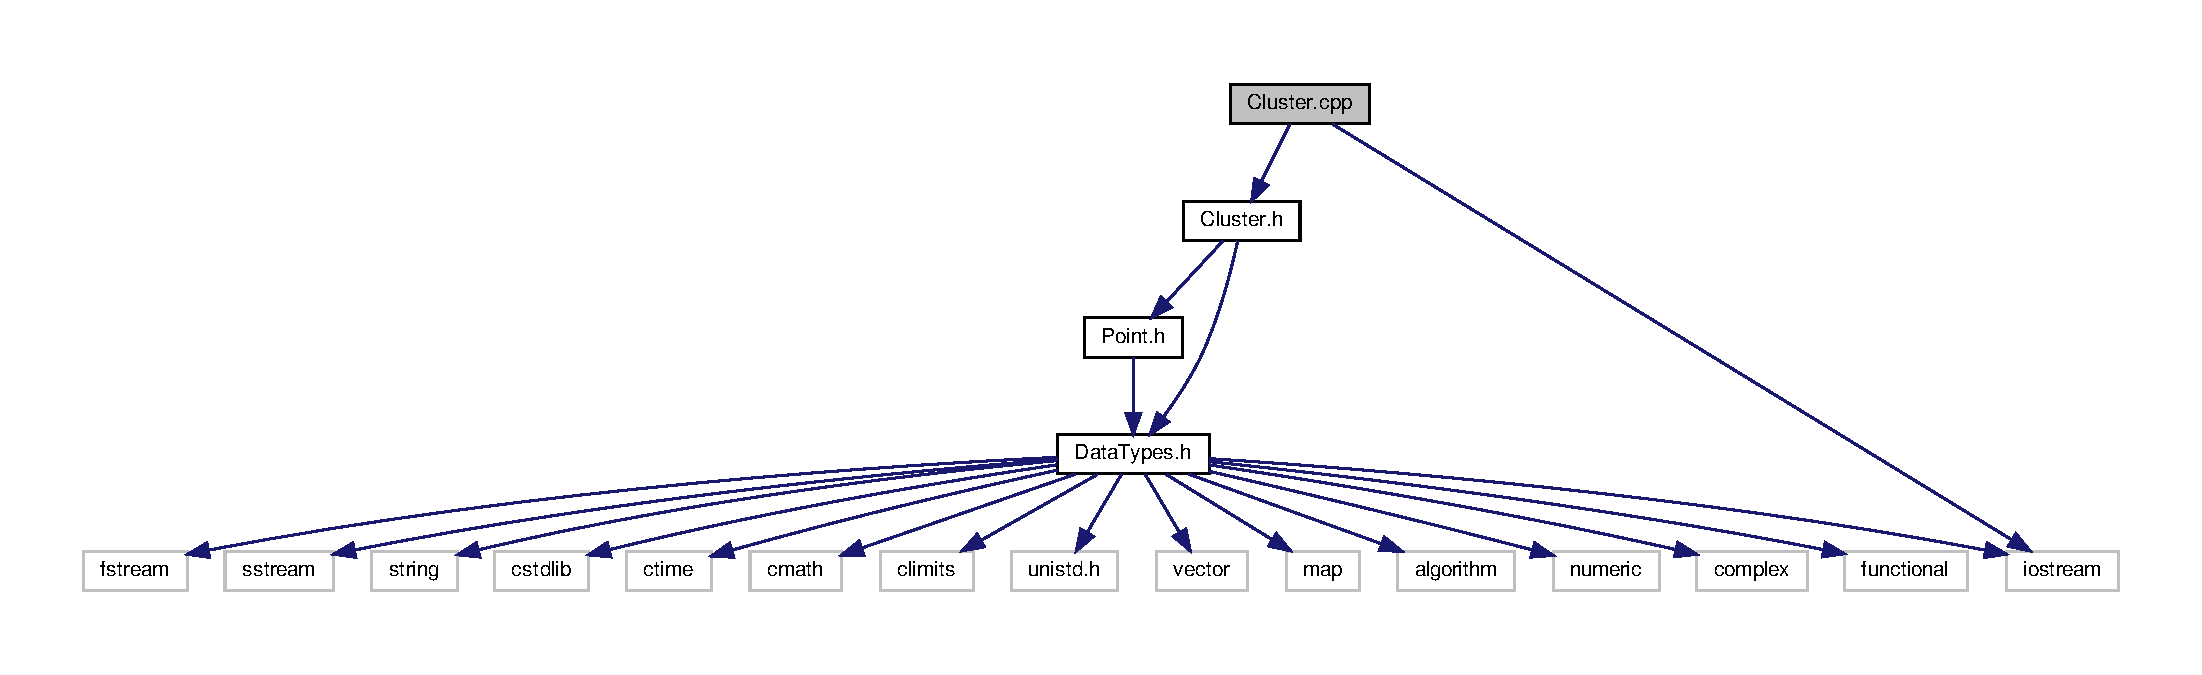
\includegraphics[width=350pt]{_cluster_8cpp__incl}
\end{center}
\end{figure}

\section{Cluster.\+h File Reference}
\label{_cluster_8h}\index{Cluster.\+h@{Cluster.\+h}}
{\ttfamily \#include \char`\"{}Data\+Types.\+h\char`\"{}}\newline
{\ttfamily \#include \char`\"{}Point.\+h\char`\"{}}\newline
\subsection*{Classes}
\begin{DoxyCompactItemize}
\item 
class \textbf{ Cluster}
\end{DoxyCompactItemize}

\section{D\+:\textbackslash{}Visual\+Studio2015\+Projects\textbackslash{}Fuzzy\+C\+Means\textbackslash{}Fuzzy\+C\+Means\textbackslash{}doc/html/dynsections.js File Reference}
\label{dynsections_8js}\index{D\+:\textbackslash{}\+Visual\+Studio2015\+Projects\textbackslash{}\+Fuzzy\+C\+Means\textbackslash{}\+Fuzzy\+C\+Means\textbackslash{}doc/html/dynsections.\+js@{D\+:\textbackslash{}\+Visual\+Studio2015\+Projects\textbackslash{}\+Fuzzy\+C\+Means\textbackslash{}\+Fuzzy\+C\+Means\textbackslash{}doc/html/dynsections.\+js}}

\section{D\+:\textbackslash{}Visual\+Studio2015\+Projects\textbackslash{}Fuzzy\+C\+Means\textbackslash{}Fuzzy\+C\+Means\textbackslash{}doc/html/jquery.js File Reference}
\label{jquery_8js}\index{D\+:\textbackslash{}\+Visual\+Studio2015\+Projects\textbackslash{}\+Fuzzy\+C\+Means\textbackslash{}\+Fuzzy\+C\+Means\textbackslash{}doc/html/jquery.\+js@{D\+:\textbackslash{}\+Visual\+Studio2015\+Projects\textbackslash{}\+Fuzzy\+C\+Means\textbackslash{}\+Fuzzy\+C\+Means\textbackslash{}doc/html/jquery.\+js}}

\section{D\+:\textbackslash{}Visual\+Studio2015\+Projects\textbackslash{}Fuzzy\+C\+Means\textbackslash{}Fuzzy\+C\+Means\textbackslash{}doc/html/menu.js File Reference}
\label{menu_8js}\index{D\+:\textbackslash{}\+Visual\+Studio2015\+Projects\textbackslash{}\+Fuzzy\+C\+Means\textbackslash{}\+Fuzzy\+C\+Means\textbackslash{}doc/html/menu.\+js@{D\+:\textbackslash{}\+Visual\+Studio2015\+Projects\textbackslash{}\+Fuzzy\+C\+Means\textbackslash{}\+Fuzzy\+C\+Means\textbackslash{}doc/html/menu.\+js}}

\section{D\+:\textbackslash{}Visual\+Studio2015\+Projects\textbackslash{}Fuzzy\+C\+Means\textbackslash{}Fuzzy\+C\+Means\textbackslash{}doc/html/menudata.js File Reference}
\label{menudata_8js}\index{D\+:\textbackslash{}\+Visual\+Studio2015\+Projects\textbackslash{}\+Fuzzy\+C\+Means\textbackslash{}\+Fuzzy\+C\+Means\textbackslash{}doc/html/menudata.\+js@{D\+:\textbackslash{}\+Visual\+Studio2015\+Projects\textbackslash{}\+Fuzzy\+C\+Means\textbackslash{}\+Fuzzy\+C\+Means\textbackslash{}doc/html/menudata.\+js}}

\section{D\+:\textbackslash{}Visual\+Studio2015\+Projects\textbackslash{}Fuzzy\+C\+Means\textbackslash{}Fuzzy\+C\+Means\textbackslash{}doc/html/navtree.js File Reference}
\label{navtree_8js}\index{D\+:\textbackslash{}\+Visual\+Studio2015\+Projects\textbackslash{}\+Fuzzy\+C\+Means\textbackslash{}\+Fuzzy\+C\+Means\textbackslash{}doc/html/navtree.\+js@{D\+:\textbackslash{}\+Visual\+Studio2015\+Projects\textbackslash{}\+Fuzzy\+C\+Means\textbackslash{}\+Fuzzy\+C\+Means\textbackslash{}doc/html/navtree.\+js}}

\section{D\+:\textbackslash{}Visual\+Studio2015\+Projects\textbackslash{}Fuzzy\+C\+Means\textbackslash{}Fuzzy\+C\+Means\textbackslash{}doc/html/navtreedata.js File Reference}
\label{navtreedata_8js}\index{D\+:\textbackslash{}\+Visual\+Studio2015\+Projects\textbackslash{}\+Fuzzy\+C\+Means\textbackslash{}\+Fuzzy\+C\+Means\textbackslash{}doc/html/navtreedata.\+js@{D\+:\textbackslash{}\+Visual\+Studio2015\+Projects\textbackslash{}\+Fuzzy\+C\+Means\textbackslash{}\+Fuzzy\+C\+Means\textbackslash{}doc/html/navtreedata.\+js}}

\section{D\+:\textbackslash{}Visual\+Studio2015\+Projects\textbackslash{}Fuzzy\+C\+Means\textbackslash{}Fuzzy\+C\+Means\textbackslash{}doc/html/navtreeindex0.js File Reference}
\label{navtreeindex0_8js}\index{D\+:\textbackslash{}\+Visual\+Studio2015\+Projects\textbackslash{}\+Fuzzy\+C\+Means\textbackslash{}\+Fuzzy\+C\+Means\textbackslash{}doc/html/navtreeindex0.\+js@{D\+:\textbackslash{}\+Visual\+Studio2015\+Projects\textbackslash{}\+Fuzzy\+C\+Means\textbackslash{}\+Fuzzy\+C\+Means\textbackslash{}doc/html/navtreeindex0.\+js}}

\section{D\+:\textbackslash{}Visual\+Studio2015\+Projects\textbackslash{}Fuzzy\+C\+Means\textbackslash{}Fuzzy\+C\+Means\textbackslash{}doc/html/resize.js File Reference}
\label{resize_8js}\index{D\+:\textbackslash{}\+Visual\+Studio2015\+Projects\textbackslash{}\+Fuzzy\+C\+Means\textbackslash{}\+Fuzzy\+C\+Means\textbackslash{}doc/html/resize.\+js@{D\+:\textbackslash{}\+Visual\+Studio2015\+Projects\textbackslash{}\+Fuzzy\+C\+Means\textbackslash{}\+Fuzzy\+C\+Means\textbackslash{}doc/html/resize.\+js}}

\section{D\+:\textbackslash{}Visual\+Studio2015\+Projects\textbackslash{}Fuzzy\+C\+Means\textbackslash{}Fuzzy\+C\+Means\textbackslash{}doc/html/search/search.js File Reference}
\label{search_8js}\index{D\+:\textbackslash{}\+Visual\+Studio2015\+Projects\textbackslash{}\+Fuzzy\+C\+Means\textbackslash{}\+Fuzzy\+C\+Means\textbackslash{}doc/html/search/search.\+js@{D\+:\textbackslash{}\+Visual\+Studio2015\+Projects\textbackslash{}\+Fuzzy\+C\+Means\textbackslash{}\+Fuzzy\+C\+Means\textbackslash{}doc/html/search/search.\+js}}

\section{D\+:\textbackslash{}Visual\+Studio2015\+Projects\textbackslash{}Fuzzy\+C\+Means\textbackslash{}Fuzzy\+C\+Means\textbackslash{}doc/html/search/searchdata.js File Reference}
\label{searchdata_8js}\index{D\+:\textbackslash{}\+Visual\+Studio2015\+Projects\textbackslash{}\+Fuzzy\+C\+Means\textbackslash{}\+Fuzzy\+C\+Means\textbackslash{}doc/html/search/searchdata.\+js@{D\+:\textbackslash{}\+Visual\+Studio2015\+Projects\textbackslash{}\+Fuzzy\+C\+Means\textbackslash{}\+Fuzzy\+C\+Means\textbackslash{}doc/html/search/searchdata.\+js}}

\section{Data\+Types.\+h File Reference}
\label{_data_types_8h}\index{Data\+Types.\+h@{Data\+Types.\+h}}
{\ttfamily \#include $<$iostream$>$}\newline
{\ttfamily \#include $<$fstream$>$}\newline
{\ttfamily \#include $<$sstream$>$}\newline
{\ttfamily \#include $<$string$>$}\newline
{\ttfamily \#include $<$cstdlib$>$}\newline
{\ttfamily \#include $<$ctime$>$}\newline
{\ttfamily \#include $<$cmath$>$}\newline
{\ttfamily \#include $<$climits$>$}\newline
{\ttfamily \#include $<$unistd.\+h$>$}\newline
{\ttfamily \#include $<$vector$>$}\newline
{\ttfamily \#include $<$map$>$}\newline
{\ttfamily \#include $<$algorithm$>$}\newline
{\ttfamily \#include $<$numeric$>$}\newline
{\ttfamily \#include $<$complex$>$}\newline
{\ttfamily \#include $<$functional$>$}\newline
\subsection*{Typedefs}
\begin{DoxyCompactItemize}
\item 
typedef std\+::vector$<$ float $>$ \textbf{ Float\+Vector}
\item 
typedef std\+::vector$<$ \textbf{ Float\+Vector} $>$ \textbf{ Float\+Vector2D}
\item 
typedef std\+::vector$<$ double $>$ \textbf{ Double\+Vector}
\item 
typedef std\+::vector$<$ \textbf{ Double\+Vector} $>$ \textbf{ Double\+Vector2D}
\item 
typedef std\+::vector$<$ int $>$ \textbf{ Int\+Vector}
\item 
typedef std\+::vector$<$ \textbf{ Int\+Vector} $>$ \textbf{ Int\+Vector2D}
\item 
typedef std\+::vector$<$ std\+::string $>$ \textbf{ String\+Vector}
\item 
typedef std\+::vector$<$ \textbf{ String\+Vector} $>$ \textbf{ String\+Vector2D}
\item 
typedef std\+::pair$<$ int, int $>$ \textbf{ Int\+Int\+Pair}
\item 
typedef std\+::pair$<$ int, float $>$ \textbf{ Int\+Float\+Pair}
\item 
typedef std\+::map$<$ int, int $>$ \textbf{ Int\+Int\+Map}
\item 
typedef std\+::map$<$ int, \textbf{ Int\+Vector} $>$ \textbf{ Int\+Int\+Vector\+Map}
\item 
typedef std\+::map$<$ int, \textbf{ Float\+Vector} $>$ \textbf{ Int\+Float\+Vector\+Map}
\end{DoxyCompactItemize}


\subsection{Typedef Documentation}
\mbox{\label{_data_types_8h_a82f6bc76e1c7a0f51bf3e95ad5d3c590}} 
\index{Data\+Types.\+h@{Data\+Types.\+h}!Double\+Vector@{Double\+Vector}}
\index{Double\+Vector@{Double\+Vector}!Data\+Types.\+h@{Data\+Types.\+h}}
\subsubsection{Double\+Vector}
{\footnotesize\ttfamily typedef std\+::vector$<$double$>$ \textbf{ Double\+Vector}}



Definition at line 25 of file Data\+Types.\+h.

\mbox{\label{_data_types_8h_a7e70d37182fdafec492c4dd396c9698c}} 
\index{Data\+Types.\+h@{Data\+Types.\+h}!Double\+Vector2D@{Double\+Vector2D}}
\index{Double\+Vector2D@{Double\+Vector2D}!Data\+Types.\+h@{Data\+Types.\+h}}
\subsubsection{Double\+Vector2D}
{\footnotesize\ttfamily typedef std\+::vector$<$\textbf{ Double\+Vector}$>$ \textbf{ Double\+Vector2D}}



Definition at line 26 of file Data\+Types.\+h.

\mbox{\label{_data_types_8h_a64be07a13efb96ba9d376c4cbc6f501e}} 
\index{Data\+Types.\+h@{Data\+Types.\+h}!Float\+Vector@{Float\+Vector}}
\index{Float\+Vector@{Float\+Vector}!Data\+Types.\+h@{Data\+Types.\+h}}
\subsubsection{Float\+Vector}
{\footnotesize\ttfamily typedef std\+::vector$<$float$>$ \textbf{ Float\+Vector}}



Definition at line 23 of file Data\+Types.\+h.

\mbox{\label{_data_types_8h_a90fed7f97f1803c7719d26e6f21b4de6}} 
\index{Data\+Types.\+h@{Data\+Types.\+h}!Float\+Vector2D@{Float\+Vector2D}}
\index{Float\+Vector2D@{Float\+Vector2D}!Data\+Types.\+h@{Data\+Types.\+h}}
\subsubsection{Float\+Vector2D}
{\footnotesize\ttfamily typedef std\+::vector$<$\textbf{ Float\+Vector}$>$ \textbf{ Float\+Vector2D}}



Definition at line 24 of file Data\+Types.\+h.

\mbox{\label{_data_types_8h_a3d5049745a50e0c457cb380125e045dc}} 
\index{Data\+Types.\+h@{Data\+Types.\+h}!Int\+Float\+Pair@{Int\+Float\+Pair}}
\index{Int\+Float\+Pair@{Int\+Float\+Pair}!Data\+Types.\+h@{Data\+Types.\+h}}
\subsubsection{Int\+Float\+Pair}
{\footnotesize\ttfamily typedef std\+::pair$<$int,float$>$ \textbf{ Int\+Float\+Pair}}



Definition at line 32 of file Data\+Types.\+h.

\mbox{\label{_data_types_8h_ae9ec0f616e5edddb88bd7cba63e2ea88}} 
\index{Data\+Types.\+h@{Data\+Types.\+h}!Int\+Float\+Vector\+Map@{Int\+Float\+Vector\+Map}}
\index{Int\+Float\+Vector\+Map@{Int\+Float\+Vector\+Map}!Data\+Types.\+h@{Data\+Types.\+h}}
\subsubsection{Int\+Float\+Vector\+Map}
{\footnotesize\ttfamily typedef std\+::map$<$int,\textbf{ Float\+Vector}$>$ \textbf{ Int\+Float\+Vector\+Map}}



Definition at line 35 of file Data\+Types.\+h.

\mbox{\label{_data_types_8h_a1972afbb2da11833cc5c4e7dda7936cf}} 
\index{Data\+Types.\+h@{Data\+Types.\+h}!Int\+Int\+Map@{Int\+Int\+Map}}
\index{Int\+Int\+Map@{Int\+Int\+Map}!Data\+Types.\+h@{Data\+Types.\+h}}
\subsubsection{Int\+Int\+Map}
{\footnotesize\ttfamily typedef std\+::map$<$int,int$>$ \textbf{ Int\+Int\+Map}}



Definition at line 33 of file Data\+Types.\+h.

\mbox{\label{_data_types_8h_aafe152bbcb51930b658b8a4406f4d67e}} 
\index{Data\+Types.\+h@{Data\+Types.\+h}!Int\+Int\+Pair@{Int\+Int\+Pair}}
\index{Int\+Int\+Pair@{Int\+Int\+Pair}!Data\+Types.\+h@{Data\+Types.\+h}}
\subsubsection{Int\+Int\+Pair}
{\footnotesize\ttfamily typedef std\+::pair$<$int,int$>$ \textbf{ Int\+Int\+Pair}}



Definition at line 31 of file Data\+Types.\+h.

\mbox{\label{_data_types_8h_afae9076c89b4ed1654b0f85beb47af82}} 
\index{Data\+Types.\+h@{Data\+Types.\+h}!Int\+Int\+Vector\+Map@{Int\+Int\+Vector\+Map}}
\index{Int\+Int\+Vector\+Map@{Int\+Int\+Vector\+Map}!Data\+Types.\+h@{Data\+Types.\+h}}
\subsubsection{Int\+Int\+Vector\+Map}
{\footnotesize\ttfamily typedef std\+::map$<$int,\textbf{ Int\+Vector}$>$ \textbf{ Int\+Int\+Vector\+Map}}



Definition at line 34 of file Data\+Types.\+h.

\mbox{\label{_data_types_8h_a9b8f2f96749808efd0d975e75d96a71c}} 
\index{Data\+Types.\+h@{Data\+Types.\+h}!Int\+Vector@{Int\+Vector}}
\index{Int\+Vector@{Int\+Vector}!Data\+Types.\+h@{Data\+Types.\+h}}
\subsubsection{Int\+Vector}
{\footnotesize\ttfamily typedef std\+::vector$<$int$>$ \textbf{ Int\+Vector}}



Definition at line 27 of file Data\+Types.\+h.

\mbox{\label{_data_types_8h_a2611314ab2c7ffc99f4b34f959b4723c}} 
\index{Data\+Types.\+h@{Data\+Types.\+h}!Int\+Vector2D@{Int\+Vector2D}}
\index{Int\+Vector2D@{Int\+Vector2D}!Data\+Types.\+h@{Data\+Types.\+h}}
\subsubsection{Int\+Vector2D}
{\footnotesize\ttfamily typedef std\+::vector$<$\textbf{ Int\+Vector}$>$ \textbf{ Int\+Vector2D}}



Definition at line 28 of file Data\+Types.\+h.

\mbox{\label{_data_types_8h_ab8e1ede88e2ff1c3b448334e6cbd3533}} 
\index{Data\+Types.\+h@{Data\+Types.\+h}!String\+Vector@{String\+Vector}}
\index{String\+Vector@{String\+Vector}!Data\+Types.\+h@{Data\+Types.\+h}}
\subsubsection{String\+Vector}
{\footnotesize\ttfamily typedef std\+::vector$<$std\+::string$>$ \textbf{ String\+Vector}}



Definition at line 29 of file Data\+Types.\+h.

\mbox{\label{_data_types_8h_acccc44108a5c4da23723c861fdaf8ed5}} 
\index{Data\+Types.\+h@{Data\+Types.\+h}!String\+Vector2D@{String\+Vector2D}}
\index{String\+Vector2D@{String\+Vector2D}!Data\+Types.\+h@{Data\+Types.\+h}}
\subsubsection{String\+Vector2D}
{\footnotesize\ttfamily typedef std\+::vector$<$\textbf{ String\+Vector}$>$ \textbf{ String\+Vector2D}}



Definition at line 30 of file Data\+Types.\+h.


\section{Fuzzy\+C\+Means.\+cpp File Reference}
\label{_fuzzy_c_means_8cpp}\index{Fuzzy\+C\+Means.\+cpp@{Fuzzy\+C\+Means.\+cpp}}
{\ttfamily \#include \char`\"{}Fuzzy\+C\+Means.\+h\char`\"{}}\newline
{\ttfamily \#include \char`\"{}Properties\+Parser.\+h\char`\"{}}\newline
{\ttfamily \#include \char`\"{}Math\+Func.\+h\char`\"{}}\newline
{\ttfamily \#include $<$string$>$}\newline
{\ttfamily \#include $<$sstream$>$}\newline
{\ttfamily \#include $<$fstream$>$}\newline
{\ttfamily \#include $<$iostream$>$}\newline
{\ttfamily \#include $<$ctime$>$}\newline
Include dependency graph for Fuzzy\+C\+Means.\+cpp\+:
\nopagebreak
\begin{figure}[H]
\begin{center}
\leavevmode
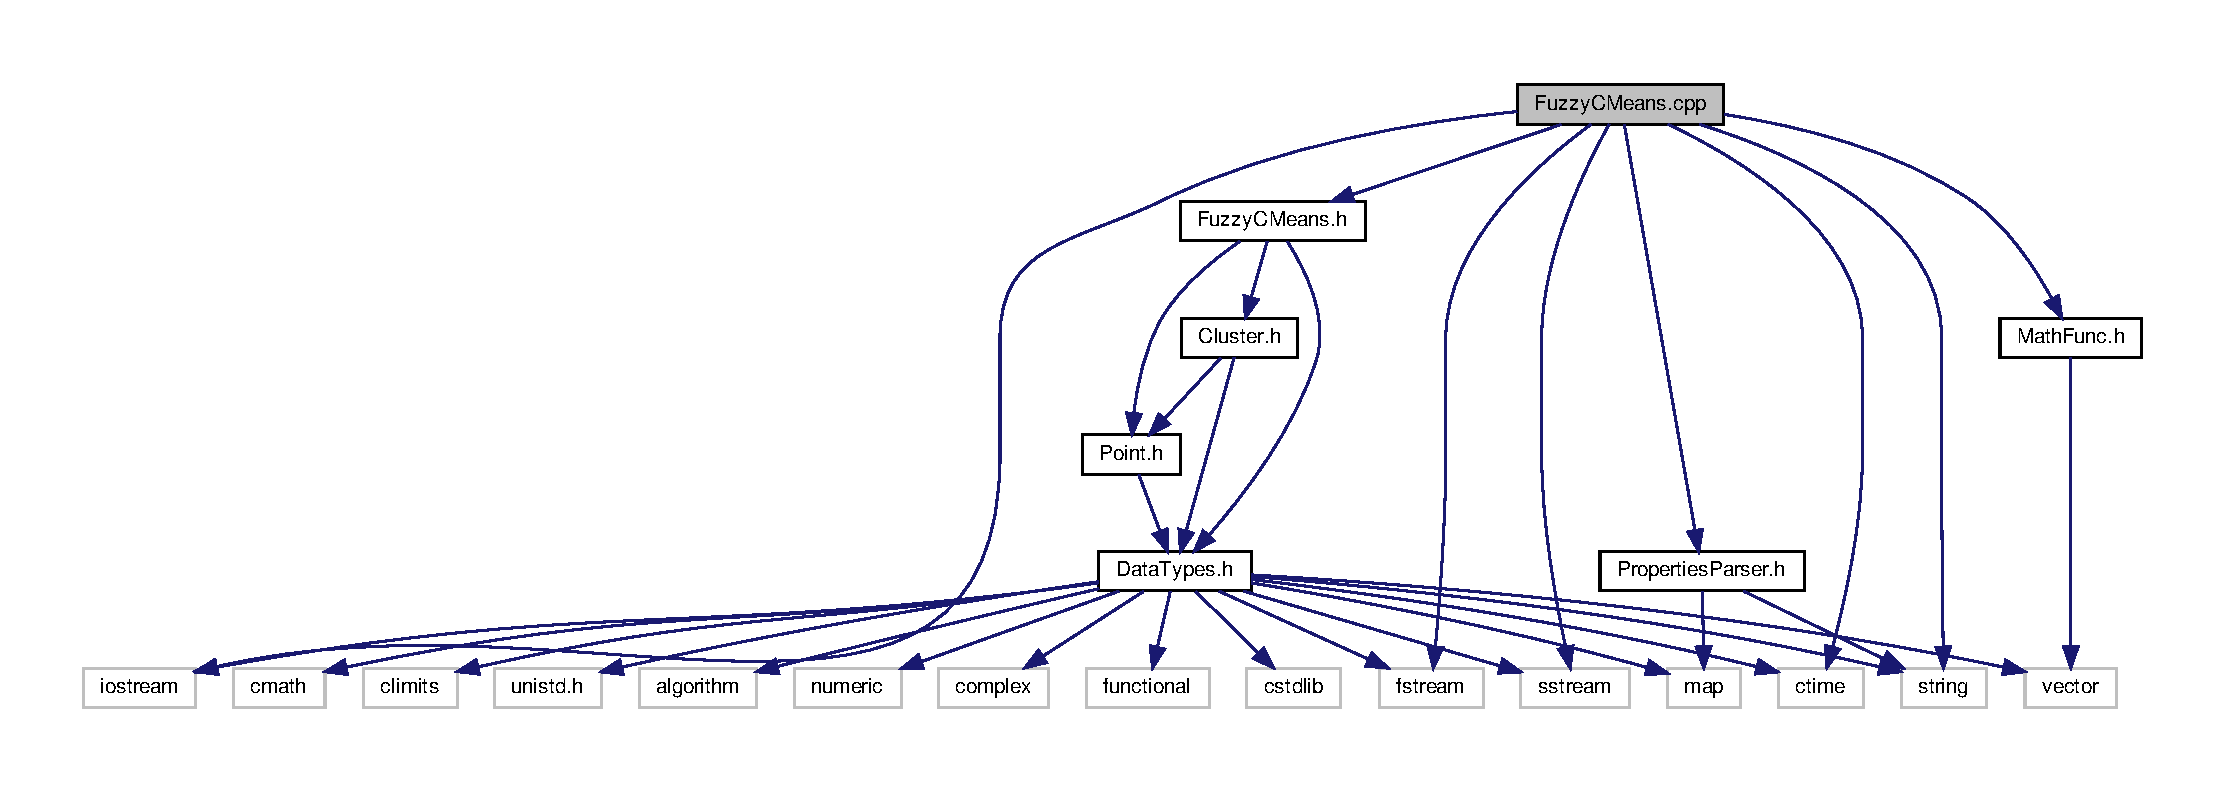
\includegraphics[width=350pt]{_fuzzy_c_means_8cpp__incl}
\end{center}
\end{figure}

\section{Fuzzy\+C\+Means.\+h File Reference}
\label{_fuzzy_c_means_8h}\index{Fuzzy\+C\+Means.\+h@{Fuzzy\+C\+Means.\+h}}
{\ttfamily \#include \char`\"{}Data\+Types.\+h\char`\"{}}\newline
{\ttfamily \#include \char`\"{}Point.\+h\char`\"{}}\newline
{\ttfamily \#include \char`\"{}Cluster.\+h\char`\"{}}\newline
\subsection*{Classes}
\begin{DoxyCompactItemize}
\item 
class \textbf{ Fuzzy\+C\+Means}
\end{DoxyCompactItemize}

\section{Generic\+Func.\+cpp File Reference}
\label{_generic_func_8cpp}\index{Generic\+Func.\+cpp@{Generic\+Func.\+cpp}}
{\ttfamily \#include \char`\"{}Generic\+Func.\+h\char`\"{}}\newline

\section{Generic\+Func.\+h File Reference}
\label{_generic_func_8h}\index{Generic\+Func.\+h@{Generic\+Func.\+h}}
{\ttfamily \#include \char`\"{}Data\+Types.\+h\char`\"{}}\newline
\subsection*{Namespaces}
\begin{DoxyCompactItemize}
\item 
 \textbf{ gf}
\end{DoxyCompactItemize}
\subsection*{Functions}
\begin{DoxyCompactItemize}
\item 
std\+::string \textbf{ gf\+::get\+Executable\+Path} ()
\item 
std\+::string \textbf{ gf\+::get\+Executable\+Path\+And\+Match\+It\+With\+Filename} (std\+::string filename)
\end{DoxyCompactItemize}

\section{main.\+cpp File Reference}
\label{main_8cpp}\index{main.\+cpp@{main.\+cpp}}
{\ttfamily \#include \char`\"{}Fuzzy\+C\+Means.\+h\char`\"{}}\newline
{\ttfamily \#include \char`\"{}Generic\+Func.\+h\char`\"{}}\newline
{\ttfamily \#include $<$string$>$}\newline
{\ttfamily \#include $<$iostream$>$}\newline
Include dependency graph for main.\+cpp\+:
\nopagebreak
\begin{figure}[H]
\begin{center}
\leavevmode
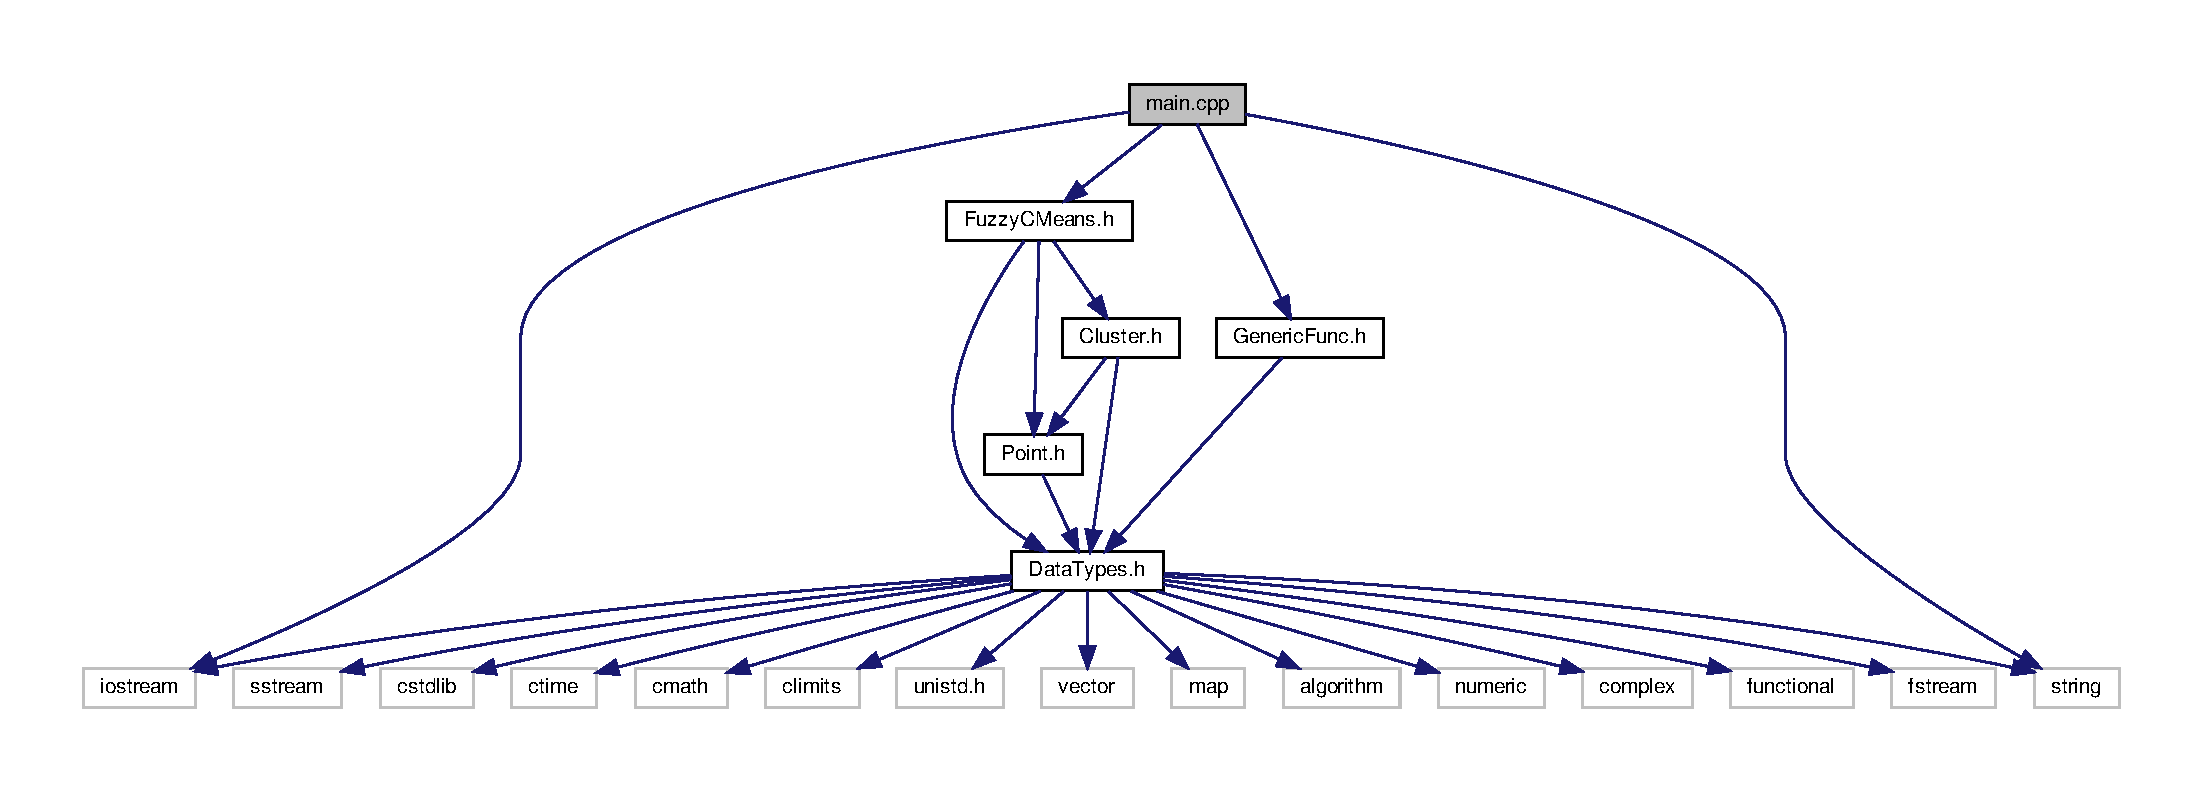
\includegraphics[width=350pt]{main_8cpp__incl}
\end{center}
\end{figure}
\subsection*{Functions}
\begin{DoxyCompactItemize}
\item 
int \textbf{ main} ()
\end{DoxyCompactItemize}


\subsection{Function Documentation}
\mbox{\label{main_8cpp_ae66f6b31b5ad750f1fe042a706a4e3d4}} 
\index{main.\+cpp@{main.\+cpp}!main@{main}}
\index{main@{main}!main.\+cpp@{main.\+cpp}}
\subsubsection{main()}
{\footnotesize\ttfamily int main (\begin{DoxyParamCaption}{ }\end{DoxyParamCaption})}



Definition at line 7 of file main.\+cpp.


\section{Math\+Func.\+h File Reference}
\label{_math_func_8h}\index{Math\+Func.\+h@{Math\+Func.\+h}}
{\ttfamily \#include $<$vector$>$}\newline
\subsection*{Namespaces}
\begin{DoxyCompactItemize}
\item 
 \textbf{ mfnc}
\end{DoxyCompactItemize}
\subsection*{Functions}
\begin{DoxyCompactItemize}
\item 
{\footnotesize template$<$typename T $>$ }\\std\+::vector$<$ T $>$ \textbf{ mfnc\+::multiply\+Vector\+By\+Constant} (const std\+::vector$<$ T $>$ \&v, const T \&c)
\item 
{\footnotesize template$<$typename T $>$ }\\std\+::vector$<$ T $>$ \textbf{ mfnc\+::add\+Vectors} (const std\+::vector$<$ T $>$ \&v\+\_\+1, const std\+::vector$<$ T $>$ \&v\+\_\+2)
\item 
{\footnotesize template$<$typename T $>$ }\\void \textbf{ mfnc\+::add\+To\+Vector} (std\+::vector$<$ T $>$ \&v, const std\+::vector$<$ T $>$ \&other\+\_\+v)
\item 
{\footnotesize template$<$typename T $>$ }\\double \textbf{ mfnc\+::compute\+Euclidean\+Distance} (const std\+::vector$<$ T $>$ \&v\+\_\+1, const std\+::vector$<$ T $>$ \&v\+\_\+2)
\end{DoxyCompactItemize}

\section{Point.\+cpp File Reference}
\label{_point_8cpp}\index{Point.\+cpp@{Point.\+cpp}}
{\ttfamily \#include \char`\"{}Point.\+h\char`\"{}}\newline
{\ttfamily \#include \char`\"{}Math\+Func.\+h\char`\"{}}\newline
{\ttfamily \#include $<$iostream$>$}\newline
{\ttfamily \#include $<$numeric$>$}\newline

\section{Point.\+h File Reference}
\label{_point_8h}\index{Point.\+h@{Point.\+h}}
{\ttfamily \#include \char`\"{}Data\+Types.\+h\char`\"{}}\newline
\subsection*{Classes}
\begin{DoxyCompactItemize}
\item 
class \textbf{ Point}
\end{DoxyCompactItemize}

\section{Properties\+Parser.\+cpp File Reference}
\label{_properties_parser_8cpp}\index{Properties\+Parser.\+cpp@{Properties\+Parser.\+cpp}}
{\ttfamily \#include \char`\"{}Properties\+Parser.\+h\char`\"{}}\newline
{\ttfamily \#include $<$fstream$>$}\newline
{\ttfamily \#include $<$sstream$>$}\newline

\section{Properties\+Parser.\+h File Reference}
\label{_properties_parser_8h}\index{Properties\+Parser.\+h@{Properties\+Parser.\+h}}
{\ttfamily \#include $<$string$>$}\newline
{\ttfamily \#include $<$map$>$}\newline
\subsection*{Classes}
\begin{DoxyCompactItemize}
\item 
class \textbf{ Properties\+Parser}
\end{DoxyCompactItemize}

\section{R\+E\+A\+D\+M\+E.\+md File Reference}
\label{_r_e_a_d_m_e_8md}\index{R\+E\+A\+D\+M\+E.\+md@{R\+E\+A\+D\+M\+E.\+md}}

%--- End generated contents ---

% Index
\backmatter
\newpage
\phantomsection
\clearemptydoublepage
\addcontentsline{toc}{chapter}{Index}
\printindex

\end{document}
